%%%%%%%%%%%%%%%%%%%
%%% 2023-04-25 %%%%
%%%%%%%%%%%%%%%%%%%
\section{Concetos de visión computacional (2023-04-25)}


\begin{frame}\frametitle{¿Qué es la visión computacional?}
  \begin{itemize}
  \item \textbf{Visión Humana: } Se puede concebir como una tarea de procesamiento de información, que obtiene significado a partir de los estímulos percibidos por los ojos.
  \item \textbf{Visión Computacional: } Desarrollo de programas de computadora que puedan \textit{interpretar} imágenes. Es decir, realizar la visión humana por medios computacionales. 
  \end{itemize}
  \begin{figure}
    \centering
    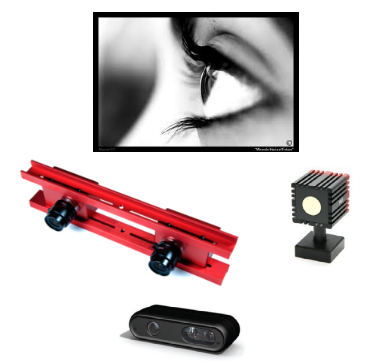
\includegraphics[width=0.5\textwidth]{Figures/ComputerVision.png}
  \end{figure}
\end{frame}

\begin{frame}\frametitle{Teoría de Marr}
“Visión es un proceso que produce, a partir de imágenes del mundo externo, una descripción que es útil para el observador y que está libre de información irrelevante.” (Marr, 1976).\\
El fenómeno de la visión lo podemos considerar como el producto de un sistema de procesamiento de información.\\

Marr propone los siguientes tres niveles de construcción de un sistema de procesamiento de información:\\
\begin{enumerate}
\item Teoría Computacional (¿Cuál es el problema por resolver?)
\item Representación y algoritmos (Estrategía usada para resolverlo)
\item Implementación (Realización física, software y hardware)
\end{enumerate}
Es decir, la visión computacional sería un proceso parecido a la visión humana, similar en los niveles computacionales y de algoritmos, pero implementado de forma diferente: en hardware de procesamiento con sensores de visión. 
\end{frame}

\begin{frame}\frametitle{Visión Computacional}
  Por lo tanto, la tarea de la Visión por computadora es la construcción de descriptores de la escena con base en características relevantes contenidas en una imagen:
  \begin{columns}
    \begin{column}{0.5\textwidth}
\begin{figure}
    \centering
    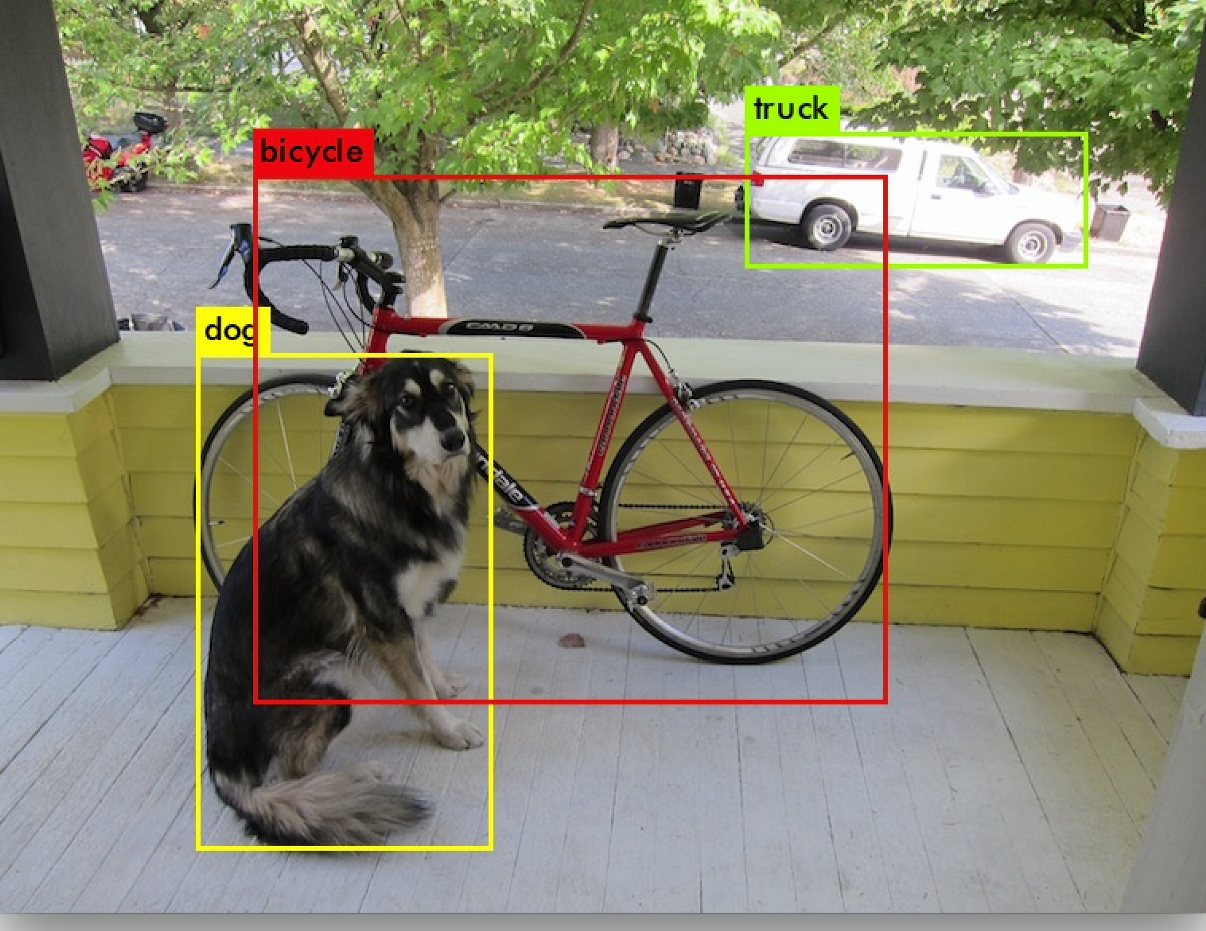
\includegraphics[width=0.8\textwidth]{Figures/YoloExample.png}
\end{figure}
    \end{column}
    \begin{column}{0.5\textwidth}
\begin{itemize}
\item Objetos
\item Formas de Superficies
\item Colores
\item Texturas
\item Movimientos
\item Iluminación
\item Reflejos
\end{itemize}
    \end{column}
    \end{columns}
\end{frame}

\begin{frame}\frametitle{Vision Computacional vs Proc de Imágenes}
\begin{enumerate}
\item Procesamiento de imagenes: Es cualquier forma de procesamiento de señales donde la entrada es una imagen, la salida puede ser otra imagen o un conjunto de características o parámetros relacionados con la misma.
\item Visión Computacional: Estudio y aplicación de métodos que permiten a las computadoras “entender” el contenido de una imagen.
\item Visión Máquina: Es la aplicación de la visión por computadora en la industria y procesos de manufactura.
\end{enumerate}

\end{frame}

\begin{frame}\frametitle{Aplicaciones}
  Tareas que se pueden hacer con visión computacional (con aplicaciones a la robótica):
  \begin{itemize}
  \item OCR (Optical Character Recognition)
  \item Detección e identificación de rostros
  \item Reconocimiento de objetos
  \item Percepción para vehículos sin conductor
  \item Reconocimiento de gestos
  \end{itemize}
  Otras aplicaciones:
  \begin{itemize}
  \item Vigilancia
  \item Imagenología médica
  \item Consultas a bases de datos de imágenes.
  \item Percepción remota
  \end{itemize}
\end{frame}


\begin{frame}\frametitle{Esquema de Visión}
  \begin{figure}
    \centering
    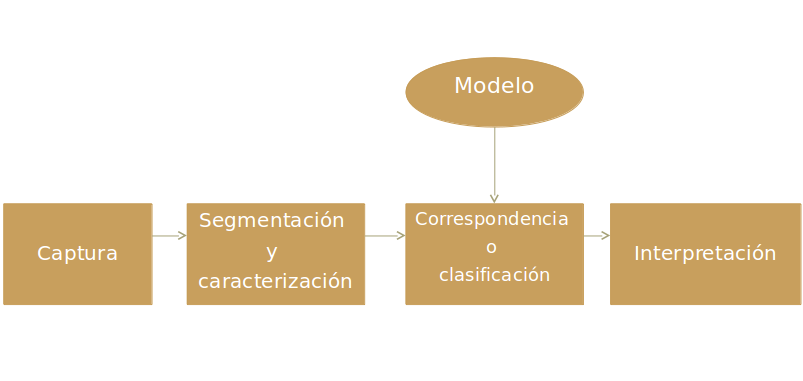
\includegraphics[width=1.0\textwidth]{Figures/VisionGeneralProcess.png}
  \end{figure}
\end{frame}


\begin{frame}\frametitle{Dificultades}

  El entorno real tiene una gran cantidad de variaciones en las imágenes de entrada.
  \begin{columns}
    \begin{column}{0.5\textwidth}
\begin{figure} %this figure will be at the right
    \centering
    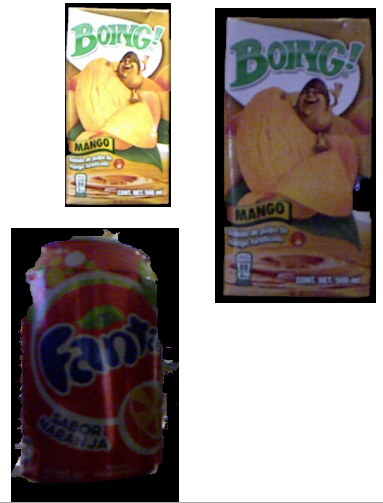
\includegraphics[width=0.5\textwidth]{Figures/ComputerVisionProblems.png}
\end{figure}
    \end{column}
    \begin{column}{0.5\textwidth}
\begin{enumerate}
\item Iluminación
\item Orientación
\item Oclusión
\item Escala
\item Ruido
\item Desenfoque
\end{enumerate}
    \end{column}
  \end{columns}
\end{frame}

\begin{frame}\frametitle{Hardware y Software}
La computación con imágenes tiene mas de 30 años, sin embargo, en los últimos años, se ha incrementado considerablemente su desarrollo debido a:
\begin{enumerate}
\item Decremento en los precios 
\item Memoria con gran capacidad
\item Procesadores de propósito general de alta velocidad.
\item Existen scanners o camaras digitales que pueden ser utilizados para procesar imágenes propias.
\item Existen bibliotecas de software que contienen subrutinas de procesamiento de imágenes (opencv).
\end{enumerate}
\end{frame}

\section[Proc Imágenes]{Procesamiento de Imágenes}
\begin{frame}\frametitle{Imágenes como funciones}
  \begin{itemize}
  \item Una imagen (en escala de grises) es una función $I(x,y)$ donde $x,y$ son variables discretas en coordenadas de imagen y la función $I$ es intensidad luminosa.
    \item Las imágenes también pueden considerarse como arreglos bidimensionales de números entre un mínimo y un máximo (usualmente 0-255).
    \item Las imágenes de color son funciones vectoriales $f:\mathbb{R}^2\rightarrow \mathbb{R}^3$ donde cada componente de la función se llama canal.
%  \[I(x,y) = \left[\begin{tabular}{c}$r(x,y)$\\$g(x,y)$\\$b(x,y)$\end{tabular}\right]\]
  \end{itemize}
  \begin{figure}
    \centering
    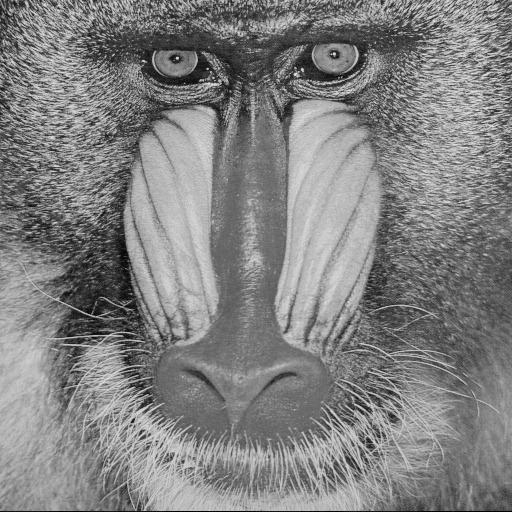
\includegraphics[width=0.3\textwidth]{Figures/baboon_grayscale.jpg}
    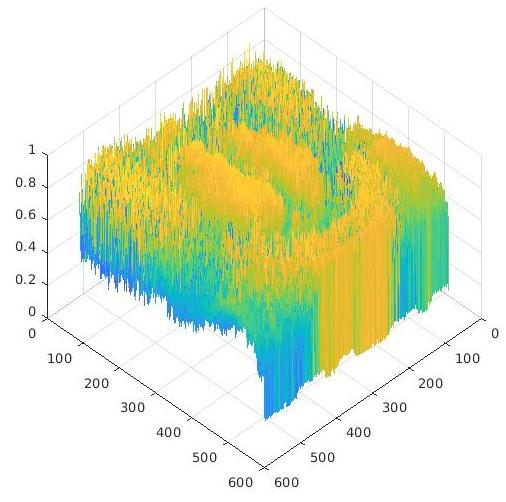
\includegraphics[width=0.35\textwidth]{Figures/BaboonPlot.jpg}
  \end{figure}
\end{frame}

\begin{frame}\frametitle{Las imágenes como funciones}
    Aunque formalmente una imagen es un mapeo $f:\mathbb{R}^2\rightarrow \mathbb{R}$, en la práctica, tanto $x,y$ como $I$ son varialbes discretas con valores entre un mínimo y un máximo.
\begin{figure}
  \centering
  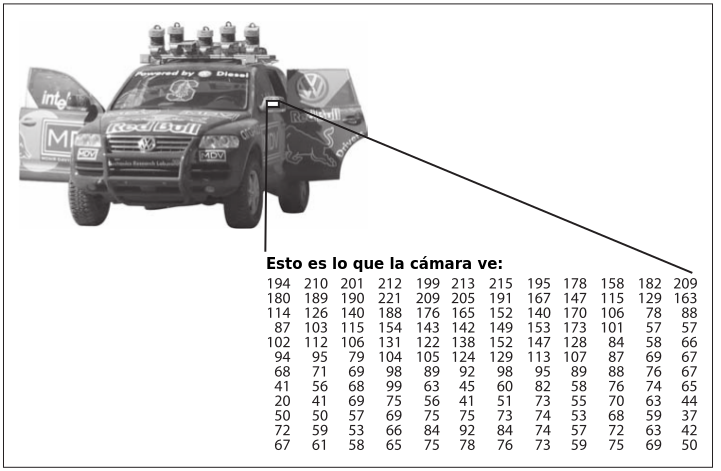
\includegraphics[width=0.45\textwidth]{Figures/ImageRepresentation.png}
\end{figure}
\end{frame}


\begin{frame}\frametitle{Operaciones básicas}
  \begin{itemize}
  \item Desfase
  \item Escalamiento
  \item Inversión en $x,y$
  \item Suma y Resta 
  \item Multiplicación
  \end{itemize}
  Ver ejercicios en Python.
\end{frame}

\begin{frame}\frametitle{Tipos de ruido}
  El ruido es una señal aleatoria $\eta(x,y)$, es decir, no sabemos cuánto vale para un punto determinado $(x,y)$ pero sí podemos caracterizarla.
  \[I_n(x,y) = I(x,y) + \eta(x,y)\]
  Existen varios tipos de ruido:
  \begin{itemize}
  \item Sal y pimienta: aleatoriamente aparecen puntos ya sea blancos o negros
  \item Ruido de impulso: aleatoriamente aparecen puntos blancos
  \item Ruido gausiano: $\eta(x,y)$ se distribuye 
  \end{itemize}
  Ver ejercicios en Python
\end{frame}

% \begin{frame}\frametitle{Tarea 11 - Herramientas de visión artificial}
% \end{frame}

\begin{frame}\frametitle{Espacios de color}
  Un espacio de color o modelo de color es una representación del color mediante un conjunto numérico de valores, generalmente tres valores. Existen varios espacios de color:
  \begin{columns}
    \begin{column}{0.5\textwidth}
      \begin{itemize}
      \item Aditivos:
        \begin{itemize}
        \item RGB
        \item HSV
        \item YCrCb
        \end{itemize}
      \item Sustractivos
        \begin{itemize}
        \item MCYK
        \end{itemize}
      \end{itemize}
    \end{column}
    \begin{column}{0.5\textwidth}
      \begin{itemize}
      \item Lineales:
        \begin{itemize}
        \item RGB
        \item CIE XYZ
        \end{itemize}
      \item No lineales
        \begin{itemize}
        \item HSV
        \item HSI 
        \end{itemize}
      \end{itemize}
    \end{column}
  \end{columns}
\end{frame}

\begin{frame}\frametitle{El espacio RGB}
  En este espacio cada color se forma mediante la suma de tres colores primarios: rojo, verde y azul. 
  \begin{figure}
    \centering
    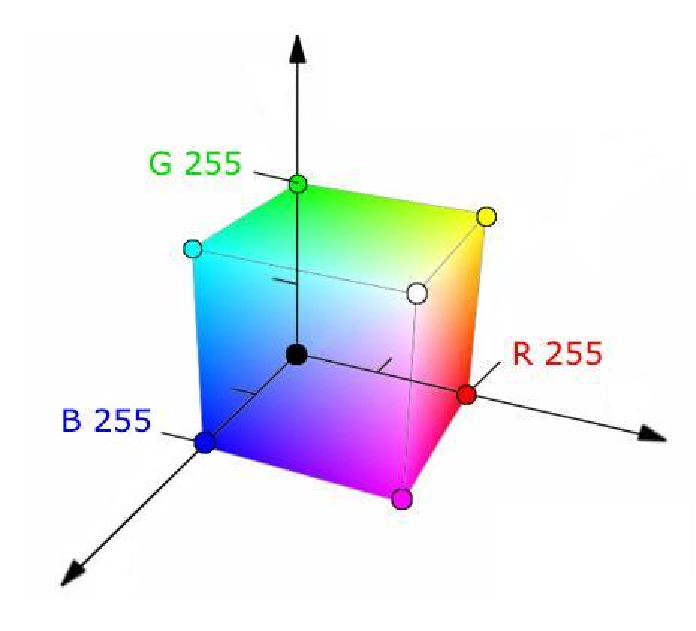
\includegraphics[width=0.33\textwidth]{Figures/RGB_model.pdf}
    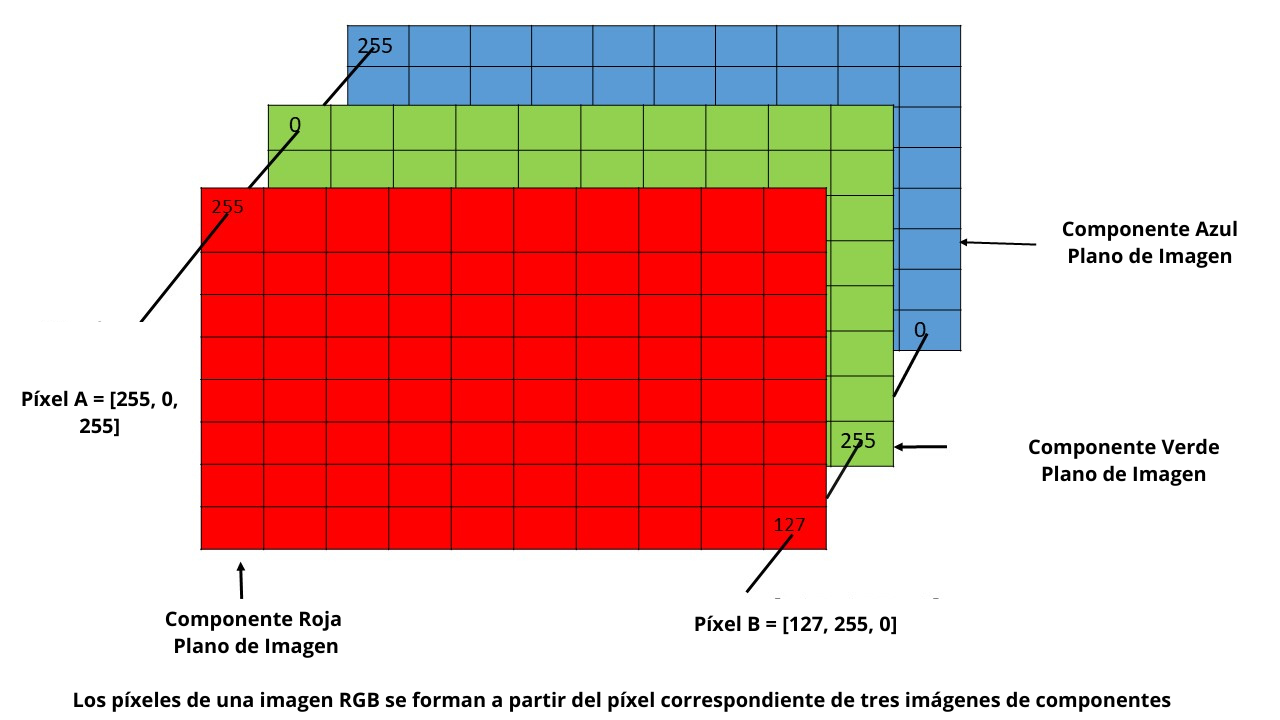
\includegraphics[width=0.5\textwidth]{Figures/rgb_pixels.png}
  \end{figure}
  En memoria, las imágenes RGB se suelen representar con arreglos de $H\times W \times 3$ donde $H$ y $W$ son el alto y ancho de la imagen respectivamente. 
\end{frame}

\begin{frame}\frametitle{El espacio HSV}
  Es un espacio de color diseñado para representar el color de una forma más similar a como lo percibe el ojo humano. El color se representa con tres valores:
  \begin{itemize}
  \item \textbf{Hue:} (Matiz) Es el atributo del color que hace que un estímulo se perciba como similar a alguno de los colores que el ojo puede percibir: rojo, amarillo, verde, azul, violeta, o una combinación de ellos.
  \item \textbf{Saturaion: } (Saturación) Es el atributo que indica qué tan colorido es un estímulo con respecto a su propio brillo.
  \item \textbf{Value: } (Valor) Atributo que indica qué tanta luz emite un estímulo. 
  \end{itemize}
  \begin{columns}
    \begin{column}{0.35\textwidth}
      \begin{figure}
        \centering
        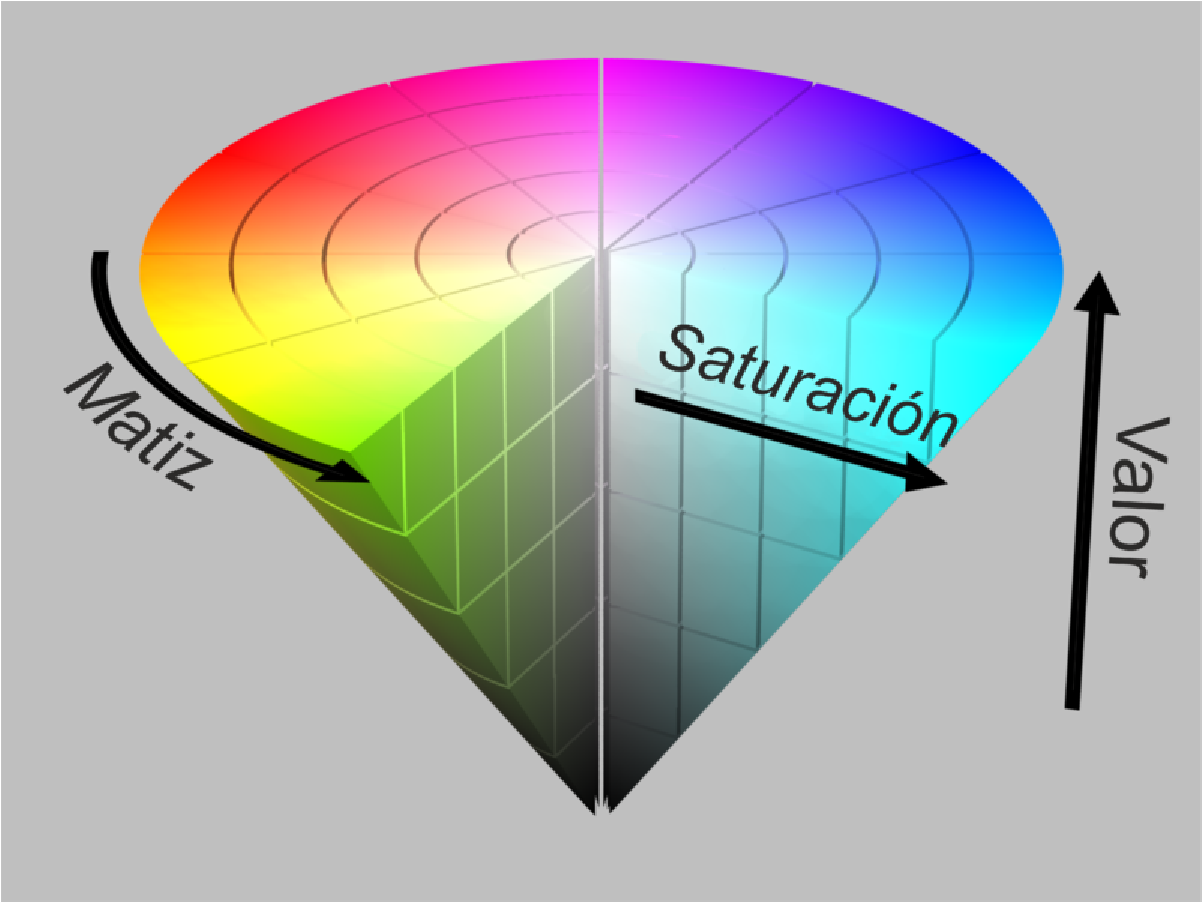
\includegraphics[width=\textwidth]{Figures/hsv_space.pdf}
      \end{figure}
    \end{column}
    \begin{column}{0.65\textwidth}
      Para obtenerlo a partir de RGB:
      \[M = \max(R,G,B)\qquad m=\min(R,G,B)\qquad C=M - m\]
      \[H = \begin{cases}\begin{tabular}{lcl}Indeterminado & si & C=0 \\ $\frac{G-B}{C}\times 60$ & si & M = R \\ $\frac{B - R}{C}\times 60$ & si & M = G \\ $\frac{R - G}{C}\times 60$ & si & M = B\end{tabular}\end{cases}\qquad V = M\]
      \[S = \begin{cases}0\qquad \textrm{si}\; V=0\\ \frac{C}{V}\qquad \textrm{en otro caso}\end{cases}\]
    \end{column}
  \end{columns}
\end{frame}

\begin{frame}\frametitle{Nubes de puntos}
  Las nubes de puntos son conjuntos de vectores que representan puntos en el espacio. Estos vectores generalmente tienen información de posición $(x,y,z)$. También pueden contener información de color $(x,y,z,r,g,b)$.
  \begin{figure}
      \centering
      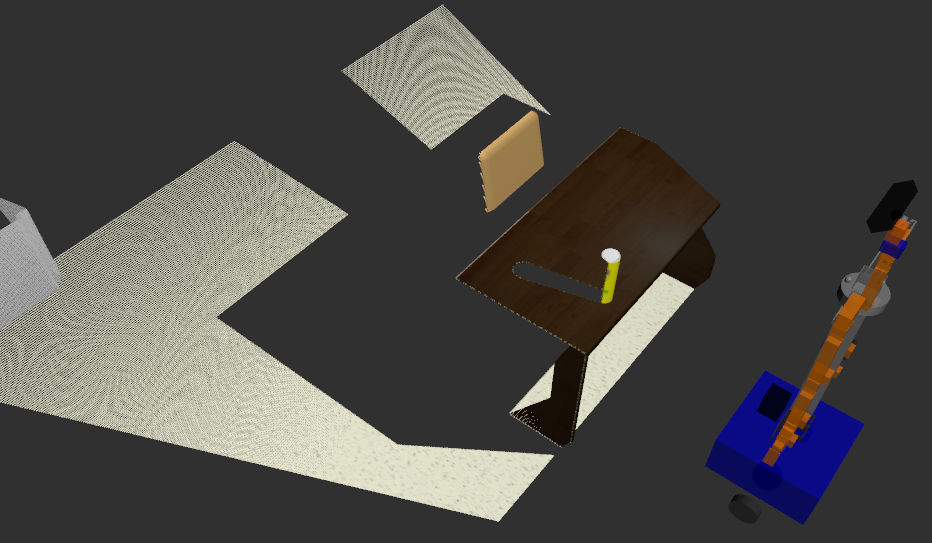
\includegraphics[width=0.5\textwidth]{Figures/CloudExample.png}
  \end{figure}
  Son útiles para determinar la posición en el espacio de los objetos reconocidos. 
\end{frame}

\begin{frame}\frametitle{OpenCV}
  \begin{itemize}
  \item OpenCV es un conjunto de bibliotecas que facilita la implementación de algoritmos de visión computacional.
  \item Se puede usar con diversos lenguajes: C++, Python, Java.
  \item En Python utiliza la biblioteca Numpy.
  \item Las imágenes se representan como matrices donde cada elemento puede ser un solo valor, o bien tres valores, dependiendo de si la imagen está en escala de grises o a color.
  \item La configuración más común es que cada pixel esté representado por tres bytes.
  \item Las nubes de puntos se representan también como matrices donde cada elemento es una terna de flotantes con la posición $(x,y,z)$.
  \end{itemize}
\end{frame}

\begin{frame}\frametitle{Segmentación por color}
  La segmentación de una imagen se refiere a obtener regiones significativas con ciertas características. En este caso, la característica es que estén en un cierto intervalo de color. Los pasos generales para esto son:
  \begin{enumerate}
  \item Transformación de la imagen del espacio BGR al HSV (función \texttt{cvtColor})
  \item Obtención de aquellos pixeles que están en un rango de color (función \texttt{inRange})
%  \item Eliminación de \textit{outliers}, generalmente con operadores morfológicos (funciones \texttt{erode} y \texttt{dilate})
  \item Obtención del centroide de la región (funciones \texttt{findNonZero} y \texttt{mean})
  \item Si se dispone de una nube de puntos, se puede obtener la posición $(x,y,z)$ del centroide de la región segementada. 
  \end{enumerate}
\end{frame}

\begin{frame}\frametitle{Práctica 06 - Segmentación por color}
  \begin{enumerate}
  % \item Investigar los siguientes conceptos:
  %   \begin{itemize}
  %   \item Espacios de color RGB y HSV
  %   \item Segmentación de imágenes
  %   \item Nubes de puntos
  %   \end{itemize}
  \item En el archivo \texttt{catkin\_ws/src/students/scripts/practice06.py}, en la función \texttt{segment\_by\_color}, realice lo siguiente:
    \begin{enumerate}
    \item Defina dos límites superiores y dos límites inferiores, en el espacio de color HSV, para segmentar las latas que se encuentran sobre el escritorio simulado.
    \item Transforme la imagen del espacio BGR al espacio HSV mediante la función \texttt{cvtColor} de OpenCV.
    \item Determine los pixeles de la imagen que pertenecen al rango de color elegido mediante la fucion \texttt{inRange} de OpenCV.
    \item Encuentre los índices de los pixeles que pertenecen al rango de color con la función \texttt{findNonZero} de OpenCV.
    \item Utilizando los índices anteriores y la nube de puntos, determine el centroide del objeto con el color seleccionado. 
    \end{enumerate}
  \item Ejecute la simulación con el comando \texttt{roslaunch bring\_up color\_segmentation.launch }
  \item Ejecute la práctica con el comando \texttt{rosrun students practice06.py}
  \item En la pestaña \textit{Simple Tasks} de la GUI, en el campo \textit{Find Object} teclee \texttt{pringles} o \texttt{drink}
  \item En el visualizador debe dibujarse una esfera morada sobre el centro del objeto seleccionado. 
  \end{enumerate}
\end{frame}

\begin{frame}\frametitle{Práctica 06 - Segmentación por color}
 \textbf{Entregables:}
  \begin{itemize}
  \item Código modificado en la rama correspondiente del repositorio en línea.
  \item Documento escrito con los puntos indicados al inicio del semestre
  \end{itemize}
  \textbf{Deadline: } 2023-05-16 al inicio de la clase. 
\end{frame}

